%% TEMPLATE - BASIC HEADER W/ RUNNING TITLE, PG NUM & HORIZONTAL LINE

\documentclass[12pt, letterpaper]{article}

% Packages
\usepackage[utf8]{inputenc}
\usepackage[margin=1in]{geometry}
\usepackage{fancyhdr}
\usepackage{graphicx}

% Header/Footer Config
\pagestyle{fancy}
\fancyhf{}
\fancyhead[L]{Skylar Denno}
\fancyhead[C]{TELCO Monthly Charge Data Report}
\fancyhead[R]{\thepage}
\renewcommand{\headrulewidth}{0.4pt}

\begin{document}

\section{Introduction}

TELCO is a telephone and communications services company that provides mobile phone service and the following 9 service add-ons to its customers:

\begin{table}[h]
\begin{tabular}{l}
[Base] Mobile Phone Service \\
+ Additional Lines     \\
+ Online Security      \\
+ Online Backup        \\
+ Device Protection    \\
+ Tech Support         \\
+ Streaming TV         \\
+ Stream Movies        \\
+ Internet Service     \\
+ Fiber Optic Internet
\end{tabular}
\end{table}


Customers start the base plan of just mobile phone service for 1 phone and choose to add whichever services they want. Their monthly bill changes based on which services they have added. 
	 Over a total of 7,043 customers' plans, TELCO has collected each customer's total monthly payment, as well as which of these services they have added. They want to know how much they can expect each specific add-on to increase customers' monthly charges by.
	 

\section {Methods}

The data was provided in a large comma separated value table. For each customer, there was the monthly charge of their plan, as well as the 10 indicator variables for the base and the 9 add ons. If the customer had added a specific service, their value in that column would be 1. Otherwise it would be 0.

Our features or independent variables are the 10 indicator variables corresponding to service add-ons. These are the variables we expect to produce the change in the target, or dependent variable: the user's monthly charge.

The data was first split into two groups at random: 80\% of the data went into the training set, and 20\% of the data went into the test set. A multivariable linear regression model, from Python's Scikit-learn library, was trained on the training data, and the test data was to be used to evaluate the performance of the model.

The model is a simple form of supervised machine learning which tries to fit an n-dimensional linear surface to most closely approximate all the points in the dataset. It does this by minimizing the sum of squares of the distances of to every point in the dataset from the plane. Once enough iterations have passed to have reasonably minimized this sum, the remaining linear combination of each of the features' contributions to changes in the target can be expressed as:

\[ \hat y = \omega_0 +\sum_i \omega_i x_i \]

Each $\omega_i$ is a "weight" that corresponds to its feature. For every unit increase in a feature $i$, the target (monthly charge in our case) is expected to change by $\omega_i$.

To evaluate our model's performance, we use three values (the hat represents a predicted y value, and no hat means a real value from the dataset. y bar is the average target value of the dataset):

\[ R^2 = 1 - \frac{\sum_{i}(y_i - \hat y_i)^2 }{\sum_{i}(y_i - \bar y_i)^2}\]

\[ MSE = \frac{1}{n} \sum_{i=1}^n (y_i - \hat y_i)^2 \]

\[ RMSE = \sqrt{MSE}\]

A model that is good at predicting will have an $R^2$ value close to 1. $R^2$ is the proportion of the observed variation in the target that can be explained by the selected features in the dataset. If a target depends on a lot of things, using any one feature will never give a high $R^2$ value. MSE (Mean Square Error) is just the average of the squares of the error between the predicted and actual values. RMSE (Root Mean Square Error) is the square root of that, returning the MSE to the same units as the target. We want to minimize MSE and RMSE towards 0.

\section {Results}

Training with 80\% of the data and testing with the remaining 20\% showed very good results: 

\[R2  : 0.9988533669069787 \]

\[MAE : \$^2 0.7757835407720778 \]

\[RMSE: \$ 1.0291697275218272 \]


$R^2$ tells us that over 99\% of the variation of people's monthly charges can be attributed to the presence or absence of the 10 add-ons. The model was only off by about \$1 on average during testing, between the monthly charge it predicted and the customer's actual monthly charge.

\newpage
Below is the model's $\omega_i$'s it had learned from the training. Each of these numbers is the expected dollar increase of a customer's monthly plan if they 

\begin{figure}[htbp]
   \centering
    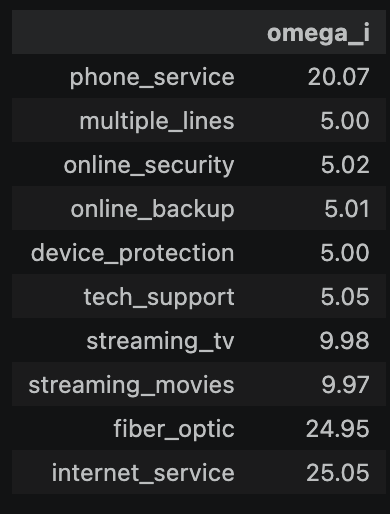
\includegraphics[width=0.3\textwidth]{coeff.png}
        
    \label{fig:my_image}
\end{figure}





\end{document}
